%-------------------------PRÉ_ÂMBULO-------------------------------------------
\documentclass[dvipdfm, a4paper, 11pt]{report}
\usepackage[brazil]{babel}
\usepackage{url}
\usepackage[utf8]{inputenc}
\usepackage{amssymb, amsmath, pxfonts}
\usepackage[normalem]{ulem} %permite sublinhar palavras
\usepackage{mathrsfs} %permite o uso de letras trabalhadas
\usepackage{graphicx}
\usepackage[usenames]{color}
\usepackage{listings}
\usepackage[]{algorithm2e} %para algoritmos
\usepackage{verbatim}%verbatim e comment
%--------------------------------------------------------------------------------
\pagestyle{empty}

\begin{document}



\vspace*{-4cm} \hspace*{-1cm} {\small
{\mbox{\begin{minipage}[t]{2.0cm}
\centerline{
\includegraphics[scale=0.25]{unimontes.eps}}
\end{minipage}}} \hspace*{1cm}
\begin{minipage}{12.0cm}{\sf \large \textbf{UNIVERSIDADE ESTADUAL DE MONTES CLAROS}}\\
{\sc Centro de Ciências Exatas e Tecnológicas}\\
{\sc Engenharia de Sistemas}\\
\end{minipage}
 \vspace*{-3mm}

\vspace{3.5cm}

\begin{center}
\LARGE{ \textbf{Sinais e Sistemas}}
\end{center}

\vspace{4cm}

\begin{center}
\huge{ \textbf{2$^o$ Trabalho}}
\end{center}

\vspace{5cm}

\Large{\uline{Luana Michelly Aparecida da Costa}}
\vspace{4cm}
\begin{center}
\normalsize{Montes Claros, 27 de maio de 2015}
\end{center}
\newpage
\normalsize{\tableofcontents }

\chapter{Introdução}\label{intro}

\section{Proposta do Trabalho}
\subsection{Função de convolução de dois sinais}
Implementar uma função que realize a convolução entre dois sinais de tempo discreto. A função
deve receber como parâmetros de entrada os dois sinais (numpy arrays) e o valor inicial da
variável independente(já que o sinal de saída somente começará a aparecer quando os dois sinais se "encontrarem", a função trabalha a partir deste ponto) e retornar o sinal resultante (numpy array) e os respectivosvalores da variável independente (numpy array).

\subsection{Realizar testes com alguns sinais}
Realize testes com alguns sinais (escolha os sinais que julgar serem interessantes), apresentando
sempre três gráficos:\\
\begin{itemize}
	\item Os sinais de entrada,
	\item O sinal resultante da convolução.
\end{itemize}
\section{Objetivos}
O objetivo principal deste trabalho, segundo o professor, é permitir que a acadêmica, 
por meio da utilização de uma ferramenta computacional, consiga compreender 
a interpretação “rebate, desloca, multiplica e soma” do somatório de convolução. 
Como objetivo secundário, tem-se o incentivo ao estudo da linguagem Python.
Além disso, toma-se como objetivo da acadêmica a continuação do estudo do \LaTeX.

\section{Descrição do Problema}\label{desc}
\subsection{Representação de sinais de tempo discreto em termos de impulsos}
Intuitivamente podemos pensar em um sinal de tempo discreto como sendo uma sequência de  impulsos individuais. Passando isso para uma afirmação matemática, tomemos o sinal da figura 1.1. Podemos considerá-lo como a soma de impulsos deslocados. Como, por exemplo, o tempo -1 pode ser representado como:\cite{oppenheim} \\
\[ x[-1]\delta[n+1] = 
\begin{cases}
x[-1], &\text{ se } n = -1, \\
0, &\text{ caso contrário }.
\end{cases}\]
\begin{figure}
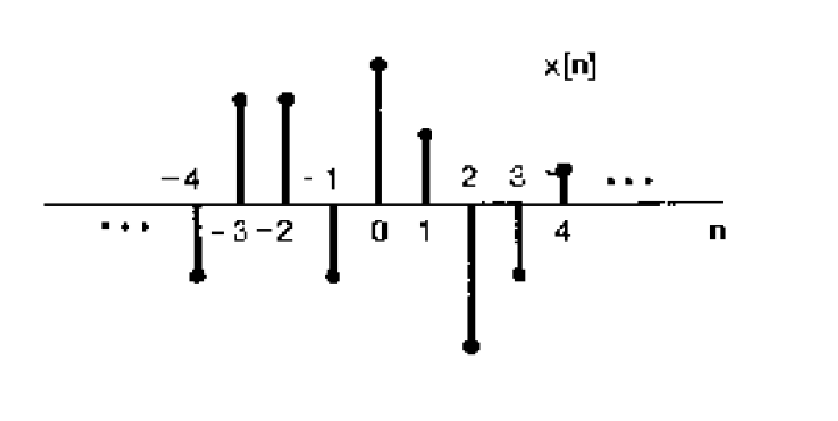
\includegraphics[scale = 0.5]{sinal_figura.eps}
\label{figura}
\caption{Sinal}
\end{figure}
Logo, podemos representar o sinal da seguinte forma:\\

\begin{gather*}
\sum_{k=-\infty}^\infty x[k]\delta[n-k].
\end{gather*}

\subsection{A resposta ao impulso e a representação da Soma de Convolução dos Sistemas LIT(Lineares e Invariantes no Tempo)}
Digamos que o operador H denote o sistema ao qual a entrada x[n] é aplicada. Então, ao usar a última equação da secção acima para o sistema, aplicando a propriedade de linearidade e sabendo que ao aplicar um impulso em um sistema a saída é a própria resposta ao impulso, temos que a resposta ao impulso para a equação em questão é:\cite{haykin}\\

\begin{gather*}
y[n] = \sum_{k=-\infty}^\infty x[k]h[n].
\end{gather*}

\chapter{Desenvolvimento}\label{desenv}

\section{Passando a ideia da solução com pseudocódigo}
Ao analisar como é formado o vetor resultante da convolução de dois sinais, pôde-se montar mais claramente um algoritmo para realizar tal função, segue abaixo o pseudo-código:\\
\\
\begin{algorithm}[H]
 \KwData{2 vetores, x e h, representando sinais de tempo discreto}
 \KwResult{1 vetor y, que é a convolução dos sinais de entrada}
 \For{i in a range(1:tamanhovetorh)}{
  \For{j in a range(1:tamanhovetorx)}{
  y[i+j] += (h[i]*x[j]);
	}
 }
 \caption{Convolução de dois sinais}
\end{algorithm}
Explicando de maneira sucinta, ao rebater o sinal cada posição do vetor x irá multiplicar no vetor vetor e aparecer na forma de soma no vetor y em uma posição a frente. Suponhamos um vetor x = [1 2 3 4] e o vetor h = [1 2 3]. Rebatemos o x, ficando [4 3 2 1]. Repare que no vetor y teremos algo como:\\
y = [x[3]*h[0] x[3]*h[0]+x[2]*h[1] ...]. Se fôssemos utilizar o vetor da maneira como o recebemos na função, podemos perceber que a primeira posição, x[0], será a que multiplicará cada elemento do vetor h e reproduzido essa multiplicação para o vetor y. A partir dos outros elementos do vetor x, haverá um deslocamento quando ele for considerado no vetor y, devido ao deslocamento do impulso comentado anteriormente.
\newpage
\section{Explicando o algoritmo passo a passo}
O código foi objetivamente comentado, então aqui acrescenta-se apenas um comentário a respeito da linha 5, que é sobre a definição do tamanho do vetor indep\_values.\\
Podemos fazer uma analogia à questão já antiga de Física que relaciona um objeto que ultrapassa outro. O caso que nos interessa aqui é o que nenhum dos objetos possa ter ser tamanho considerado desprezível, como por exemplo um trem passando por um túnel. Para calcular o tempo de ultrapassagem, é considerado o tamanho dos dois corpos. Então como nenhum dos sinais tem um tamanho desprezível, os tempos dos impulsos\(que em analogia seriam os tamanhos dos mesmos\) dos sinais são somados e subtraídos de um. Isso porque caso não sejam subtraídos seu último valor seria duplicado. Quanto à soma do valor inicial, esta ocorreu para impedir que o tamanho estabelecido seja influenciado pela determinação do início do vetor.
\small{
\begin{lstlisting}[language = python]
def Conv(x,h,valor_inicial):
	#Inicializando algumas variaveis
	lenx = len(x)
	lenh = len(h)
	indep_values = np.arange(valor_inicial, valor_inicial+lenh+lenx-1,1)
	#Mantem o tamanho do vetor, independente do valor_inicial
	y = np.zeros(lenh+lenx-1)
	for i in range(lenh):
		for j in range(lenx):
			y[i+j] = y[i+j] + (h[i]*x[j]) 
		#a medida em que os sinais vao se "interceptando", 
		#o valor de y se atualiza
	return (y, indep_values)
\end{lstlisting}
}
\newpage
\section{A escolha dos casos teste}

Ao todo foram montados seis casos teste. Em parte aleatórios, mantendo preservado o objetivo inicial ao escolhê-los.
De 1 a 3, os testes variam o tempo inicial entre negativo, positivo e nulo, respectivamente. Os outros visam corroborar 3 das propriedades da convolução. O número 4 ratifica a propriedade comutativa, o 5, a distributiva e o 6 o impulso como elemento neutro da convolução.\\
\\
Teste1 - Valor inicial negativo\\
x = [5,2,4,5,2,5,7,5]\\
h = [6,3,5,4,6]\\
tempo inicial = -4\\
\\
Teste2 - Valor inicial positivo\\
x = [6,3,5,4,6]\\
h = [1,4,2]\\
tempo inicial = 3\\
\\
Teste3 - Valor inicial nulo\\
x = [1,1,-1,0,2,-2]\\
h = [-2,1,1,1,1]\\
tempo inicial = 0\\
\\
Teste4 - Comutativa\\
x = [1,4,2]\\
h = [6,3,5,4,6]\\
tempo inicial = 0\\
\\
Teste5 - Distributiva\\
x = [6,6,6,5,2,5,7,5]\\
h = [6,3,5,4,6]\\
tempo inicial = 0\\
\\
Teste6 - Impulso como elemento neutro\\
x = [6,2,4,9,1]
h = [1]
tempo inicial = 0\\
\\
\chapter{Resultados}\label{result}
Primeiramente os vetores foram convoluídos pelo software Matlab para efeito de comparação e validação dos resultados. Logo após foram gerados os gráficos, validando o código.
\section{Gráficos gerados pelo algoritmo}
As dimensões dos gráficos foram pseudo-aleatórias, respeitando que os valores resultantes deveriam aparecer. Estão em ordem crescente dos testes como foram apresentados aqui, além de possuir um título para orientação.\\
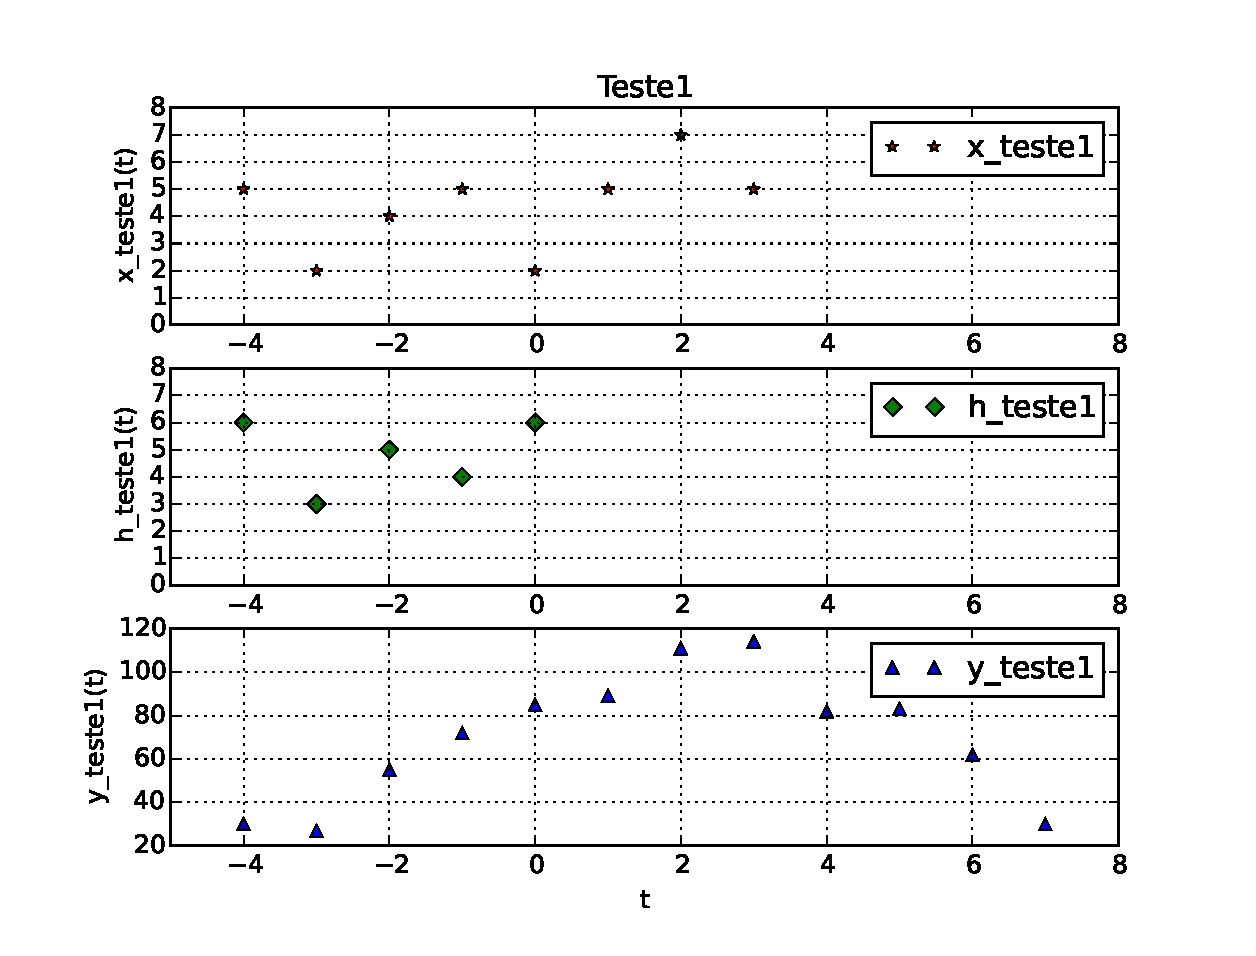
\includegraphics[scale = 0.5]{Teste1.eps}\\
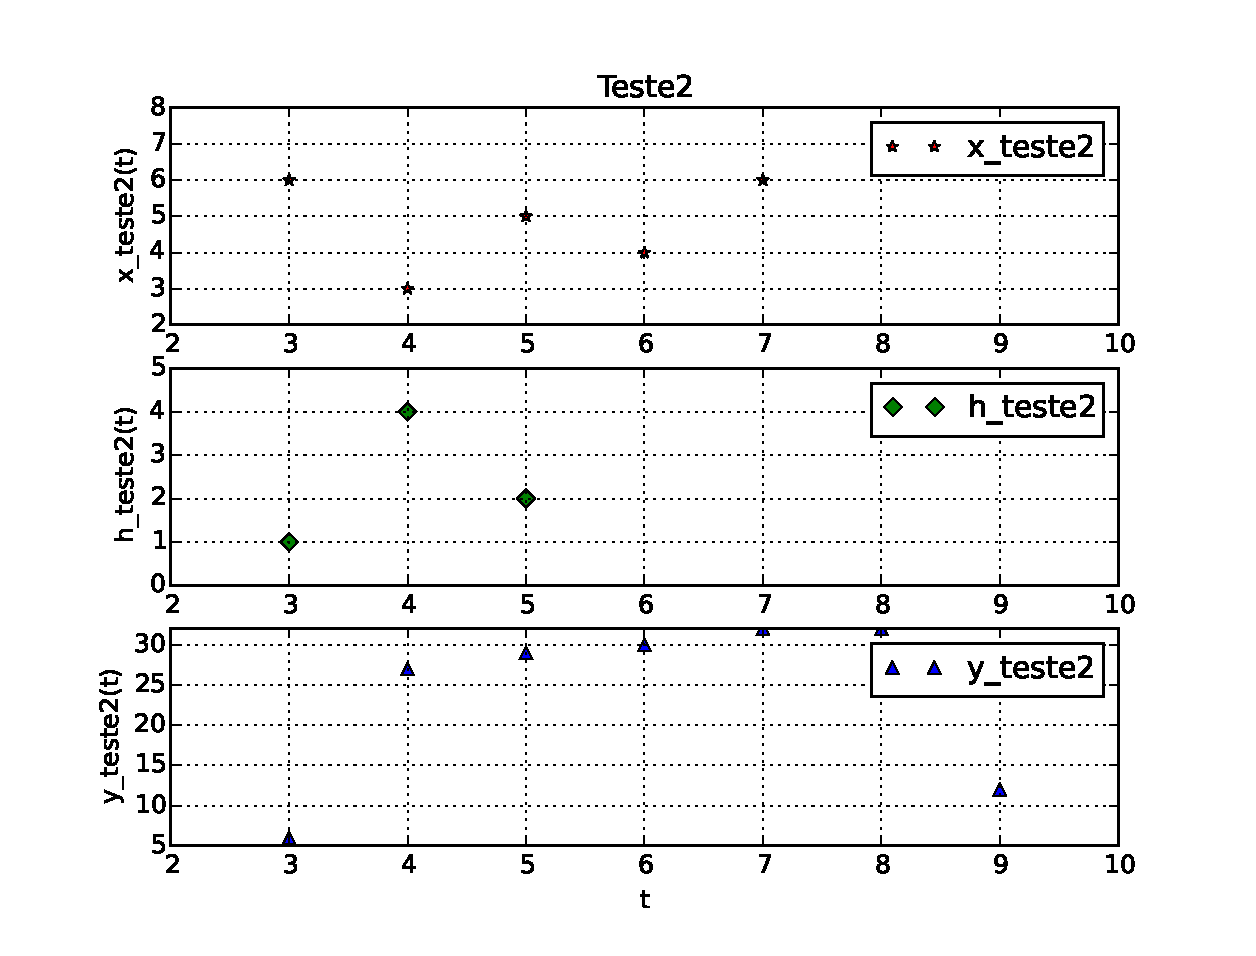
\includegraphics[scale = 0.5]{Teste2.eps}\\
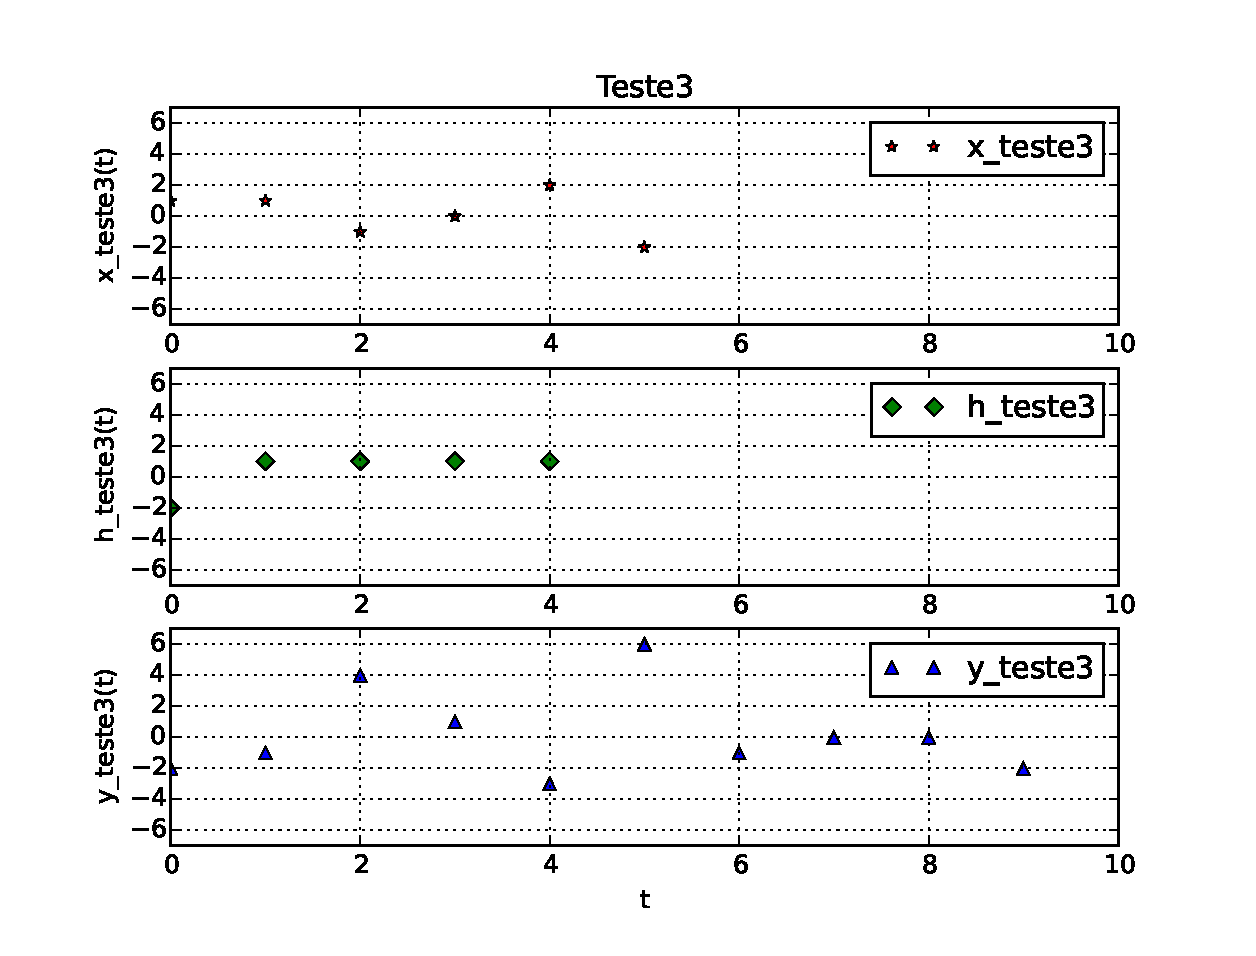
\includegraphics[scale = 0.5]{Teste3.eps}\\
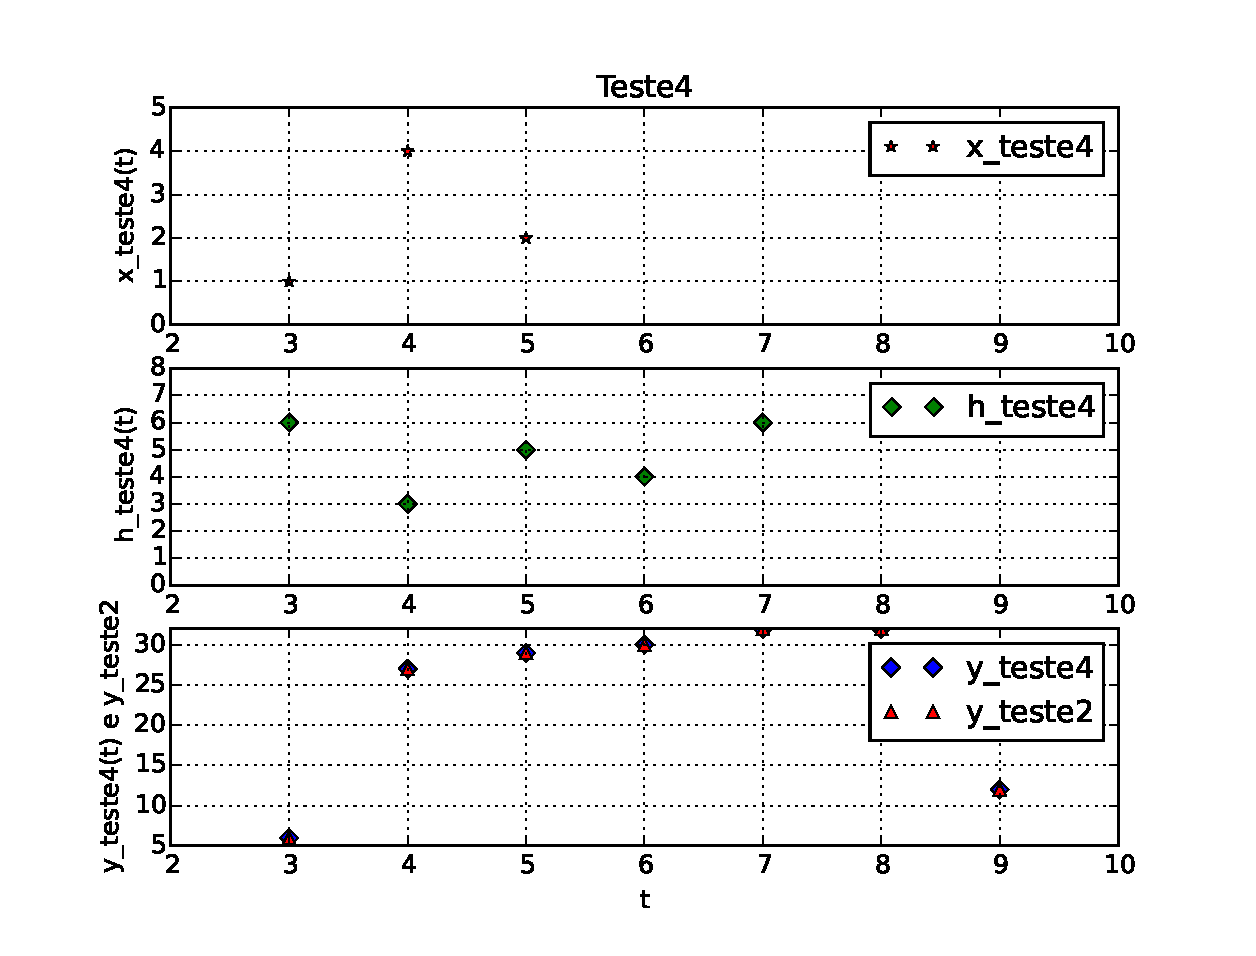
\includegraphics[scale = 0.5]{Teste4.eps}\\
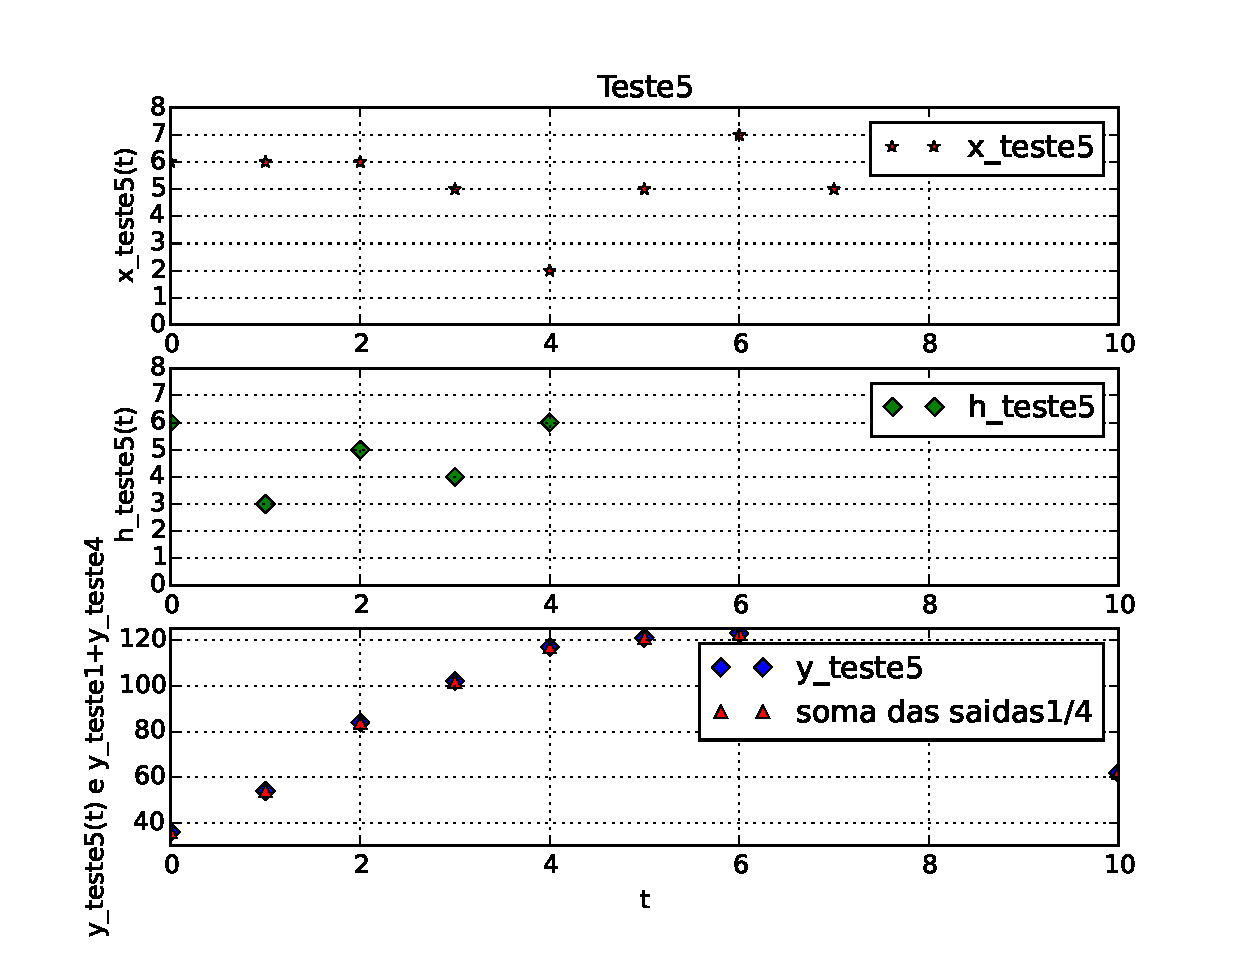
\includegraphics[scale = 0.5]{Teste5.eps}\\
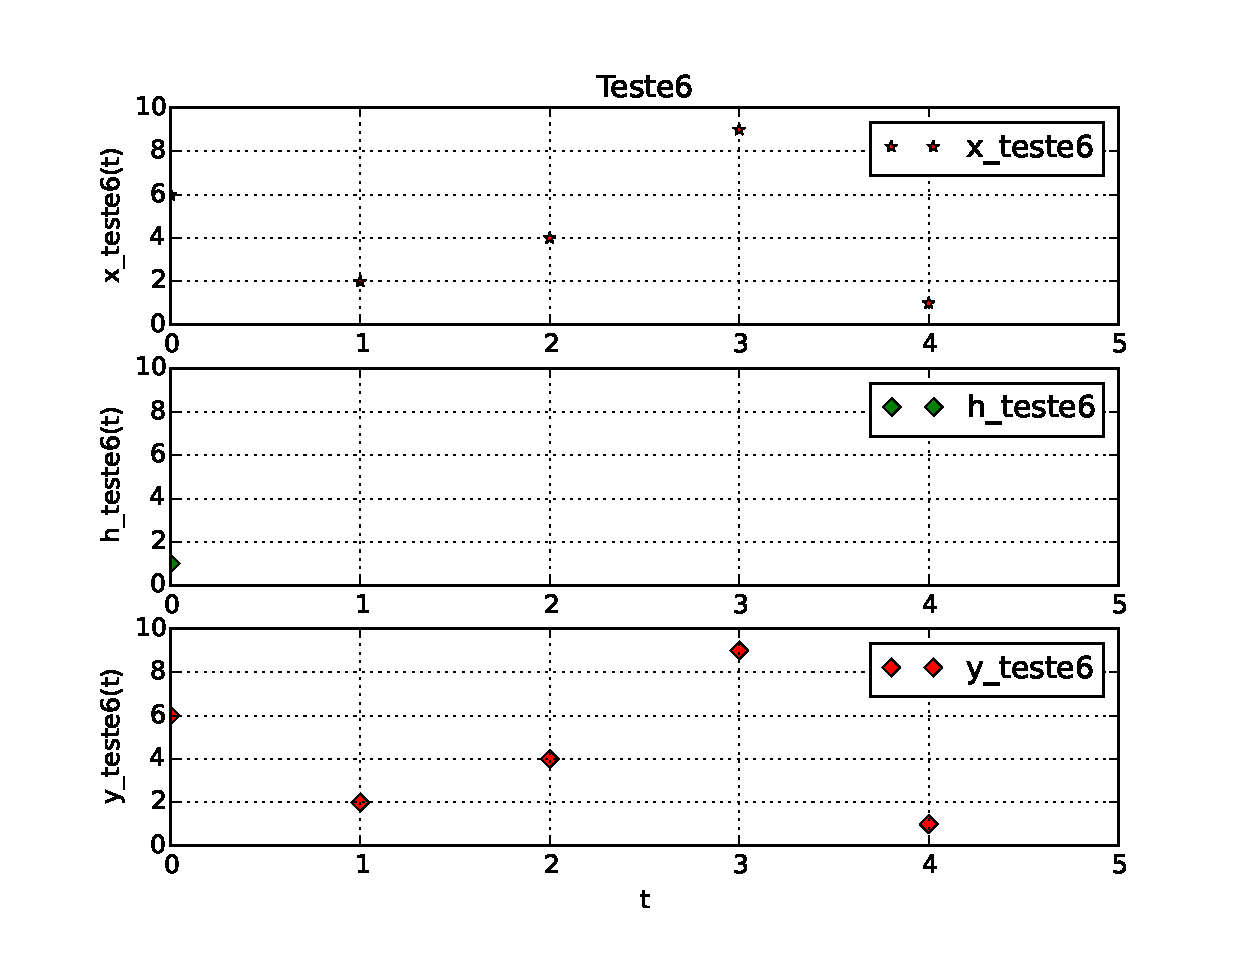
\includegraphics[scale = 0.5]{Teste6.eps}\\
\chapter{Conclusão}\label{conc}
De acordo com os resultados apresentados durante o desenvolvimento da documentação, pode-se afirmar que todos os objetivos foram cumpridos.
Quanto à elaboração da função, ela funciona adequadamente, gerando os gráficos correspondentes. O estudo das linguagens \emph{Python} e \LaTeX vem elevando para que o trabalho possa ser desenvolvido da melhor maneira possível.

\begin{thebibliography}{999}
\small{
\bibitem{np} NumPy Reference. Disponível em: $<$\url{http://docs.scipy.org/doc/numpy/reference/index.html}$>$. Acesso em: 18 de maio de 2015. 
\bibitem{matplot} Matplotlib Reference. Disponível em: $<$\url{http://matplotlib.org/contents.html}$>$. Acesso em: 18 de maio de 2015.
\bibitem{oppenheim} OPPENHEIM, A.V.;WILLSKY,A.S.;NAWAB,S.H.\emph{Signals and Systems}. 2th edition.
\bibitem{haykin} HAYKIN, S.; VEEN,B.V. \emph{Sinais e Sistemas}. Tradução: José Carlos Barbosa dos Santos. Porto Alegre, 2001
\bibitem{wolfram} Demonstração da Soma de Convolução em formato "*.cdf". Wolfram Demonstrations Project.
\bibitem{site} Vetores e matrizes com numpy. Disponível em: $<$\url{http://www.pbx-brasil.com/Pesquisa/Ferramentas/ProgramandoPython/aula112/vetoresNumpy.html}$>$. Acesso em: 18 de maio de 2015.
\bibitem{pdfaula1} Sistemas lineares e Invariantes. Universidade do Porto, Faculdade de Engenharia, 2007/2008.$<$\url{http://paginas.fe.up.pt/~mines/SS/Teoricas/SLITs/SS_slits_aula1.pdf}$>$. Acesso em: 18 de maio de 2015.
\bibitem{python_flavio}Computação científica com Python. Disponível em: $<$\url{http://www.complex.if.uff.br/_media/python_flavio.pdf}$>$. Acesso em  18 de maio de 2015.
\bibitem{mathworks}Documentação da função \textit{conv} do Matlab. Dis $<$\url{http://www.mathworks.com/help/matlab/ref/conv.html}$>$. Acesso em: 18 de maio de 2015.
\bibitem{wiki}Convolução.Disponível em: $<$\url{http://pt.wikipedia.org/wiki/Convolução}$>$. Acesso em: 18 de maio de 2015.
\bibitem{miles}MILES. Not-So-Frequently Asked Questions for \LaTeX, 2010. Disponível em: $<$\url{http://web.mit.edu/rsi/www/pdfs/ifaq.pdf}$>$ . Acesso em: 24 de maio e 2015.
\bibitem{wikibooks}Wikibooks-\LaTeX. Disponível em: $<$\url{http://en.wikibooks.org/wiki/LaTeX}$>$. Acesso em: 24 de maio de 2015.
\bibitem{brito}BRITO, Rafael.The algorithms bundle, 2009. Disponível em: $<$\url{http://repositorios.cpai.unb.br/ctan/macros/latex/contrib/algorithms/algorithms.pdf}$>$. Acesso em: 24 de maio de 2015.
}
\end{thebibliography}
\end{document}



